\chapter{Reconstruction}
\label{ch:reconstruction}

Each event within an AD is assigned a reconstructed position and energy
that take into account the pattern of PMT hits, the total light emitted,
scintillator and mineral oil optical characteristics,
spatial nonuniformity, and scintillator and electronics nonlinearity.
The reconstructed positions are used to compute the distance-time cut
to select IBD events as described in \cref{sec:DT_cut},
and are also used as inputs to the energy reconstruction
to help correct for nonuniformities in the ADs' light collection
as a function of position.
The reconstructed energy is a critical input to the \thetaot{} analysis
due to the heavy reliance on energy cuts to select IBDs and reject background.
The relative performance of ADs in reconstructing energy
is particularly important, since inconsistencies in energy reconstruction
could lead to unaccounted-for differences in efficiency,
which would bias the measurement of \thetaot.
The position reconstruction procedure will be detailed in \cref{sec:reco_position}.
Energy reconstruction, including the energy scale, determination of event energy,
and the nonuniformity and nonlinearity corrections,
will be described in \cref{sec:reco_energy}.

\section{Position}
\label{sec:reco_position}

Daya Bay uses two independent position reconstruction algorithms,
both of which rely on the pattern of charge measurements across all PMTs in an AD.
The reconstruction used in this \thetaot{} analysis is known as ``AdSimple;''
the name was inherited from a predecessor algorithm \cite{adsimple1}.
The other reconstruction is called ``AdScaled,''
in which a center-of-charge position is computed,
averaging over each PMT position weighted by the charge on the PMT,
and a parametrized correction derived from simulation
is applied to determine the reconstructed position \cite{ngd2016}.

In AdSimple,
each event's PMT charge pattern is compared to a library of \num{9600} templates
generated using a Monte Carlo simulation.
Each template represents one position on an $(r, \phi, z)$ grid
with \num{20} $r$ positions, \num{24} $\phi$ positions,
and \num{20} $z$ positions.
A $\chi^2$ is constructed to quantify the agreement between the measured charge pattern
and each of the templates:

\begin{equation}
    \chi^2(\textbf{r}_{\text{rec}}) = \sum_{i=1}^{192} -2\ln\frac{
        \text{Poisson}(N_i^{\text{obs}} \vert N_i^{\text{template}}(\textbf{r}_{\text{rec}}))
    }
    {
        \text{Poisson}(N_i^{\text{obs}} \vert N_i^{\text{obs}})
    },
\end{equation}
where $i$ indexes over PMTs,
$N_i^{\text{obs}}$ is the number of photoelectrons observed in PMT $i$,
$N_{i}^{\text{template}}(\textbf{r}_{\text{rec}})$ is the prediction
for PMT $i$ of the template for reconstructed position $\textbf{r}_{\text{rec}}$,
and $\text{Poisson}(n\vert\mu)$ is the Poisson probability
to observe $n$ counts given an expected value of $\mu$.
Once the lattice point with the least $\chi^2$ is found,
an interpolation is performed along each coordinate dimension $(r, \phi, z)$
as depicted in \cref{fig:interpolation}
to extend the domain of the $\chi^2$ function to all positions within the AD,
not just the lattice points.
The value of $\textbf{r}_{\text{rec}}$ which minimizes $\chi^2$
is used as the reconstructed position.
The distribution of reconstructed positions is shown in \cref{fig:position_map},
with artifacts of the interpolation process clearly visible.

\begin{figure}
    \centering
    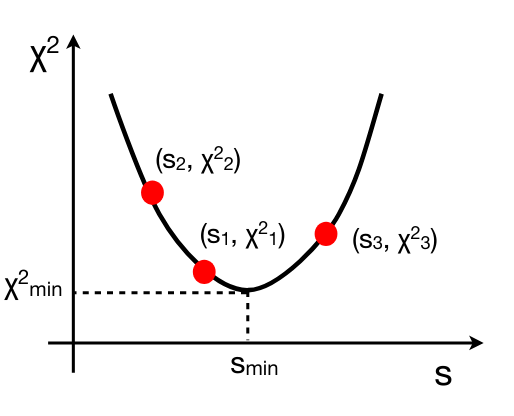
\includegraphics[width=0.4\textwidth]{ch_reconstruction/interpolation}
    \caption{
        Interpolation between grid points to obtain a more-precise position
        that minimizes the $\chi^2$ function.
        The process is repeated with $s$ representing each of the coordinates
        $r, \phi, z$.
        Figure taken from \cite{adsimple1}.
    }
    \label{fig:interpolation}
\end{figure}

\begin{figure}
    \missingfigure{Reconstructed position distribution for events in EH1-AD1}
    \caption{
        Reconstructed positions of events with energy within \SIrange{1.5}{12}{\MeV}
        in EH1-AD1.
    }
    \label{fig:position_map}
\end{figure}

\section{Energy}
\label{sec:reco_energy}

The reconstructed energy for an event is built up from the previously-described
calibration values and the observed signals in each PMT,
and then corrected for AD nonuniformity and nonlinearity.
PMT observed ADC values are converted into charges using the gain
and corrected for the single-channel nonlinearity.
The total charge on all PMTs is converted into an energy value
using the light yield measured during calibration,
and then corrected to account for any disabled PMTs
and the time-dependent spatial nonuniformity \cite{ngd2016}.
This process can be represented by the following formula:

\begin{equation}
    E_{\text{rec}} = \left(
        \sum_i f_{\text{SCNL}}\left(\frac{Q_i}{\overline{Q}_i^{\text{SPE}}(t)}\right)
    \right)
    \frac{f_{\text{act}}(t)}{N^{\text{PE}}(t)}
    f_{\text{pos}}(\textbf{r}_{\text{rec}},t),
\end{equation}
where $Q_i$ is the ADC value for PMT $i$,
$\overline{Q}_i^{\text{SPE}}(t)$ and $N^{\text{PE}}(t)$
are the gain for PMT $i$ and the light yield, respectively,
$f_{\text{SCNL}}$ is the single-channel nonlinearity correction,
and $f_{\text{act}}(t)$ and $f_{\text{pos}}(\textbf{r}_{\text{rec}},t)$
are the active PMT correction and nonuniformity correction,
described below.

The active PMT correction compensates for the loss in collected light
when a PMT must be disabled during operation \cite{ngd2016}.
On average, each PMT contributes $\nicefrac{1}{192}$ of the charge to each event.
Thus if $n$ PMTs are disabled, the measured total charge must be increased by a factor

\begin{equation}
    f_{\text{act}}(n) = \frac{192}{n}.
\end{equation}
The correction is time-dependent since the number of disabled PMTs changes with time.
\todo{Decide whether to study improved active PMT correction}

The nonuniformity correction ensures that events of a given physical energy
occurring in different regions of the AD
are assigned the same reconstructed energy.
Nonuniformities in reconstructed energy arise due to a variety of factors
including PMT light acceptance as a function of incident angle;
optical properties of the scintillator, mineral oil, and acrylic vessels;
and the orientation of PMTs with respect to the Earth's magnetic field.
The nonuniformity correction is factored into corrections based on
$r$ and $z$ position, azimuthal angle $\phi$, and time
(which also has a radial dependence):
\begin{equation}
    f_{\text{pos}}(\textbf{r}_{\text{rec}},t) =
    f_{\text{pos}}(r, z)f_{\text{pos}}(\phi)f_{\text{pos}}(r, t).
\end{equation}

Maps for the $r$--$z$ nonuniformity were constructed for each AD
by identifying neutron captures on both Gd and H,
and comparing the energy of events in a given region of the AD
to the average of the entire AD.
The AD was divided into equal-volume concentric rings
represented as squares on a plot of $z$ vs. $r^2$.
Neutron captures of spallation neutrons were selected
based on a time coincidence with a previous muon signal in the AD.
Neutron captures with energy near \SI{8}{\MeV} were assumed to be nGd captures,
and those with energy near \SI{2.2}{\MeV} were assumed to be nH.
The peak value was extracted from a fit of the respective distributions
for each pixel and for the entire sample.
\todo{What is the "average" value for LS pixels?}
The nGd peak was fit with a double-Crystal Ball function \cite{cbfunction},
and the nH peak was fit with a calorimeter function \cite{calorimeter2016}
(described in \cref{subsec:delayed}).
A correction was then applied to each event's energy based on its position:
\begin{equation}
    f_{\text{pos}}(r, z) = \frac{E_{\text{avg}}}{E_{\text{pixel}}(r,z)}.
\end{equation}
\Cref{fig:nonuniformity_map} shows the corrections $f_{\text{pos}}$ for EH1-AD1.
All ADs had similar nonuniformities, but separate corrections were still computed
for each AD.
Within an AD, the nonuniformity correction was as large as \SI{20}{\percent}
at the outer edge of the OAV (LS region).

\begin{figure}
    \centering
    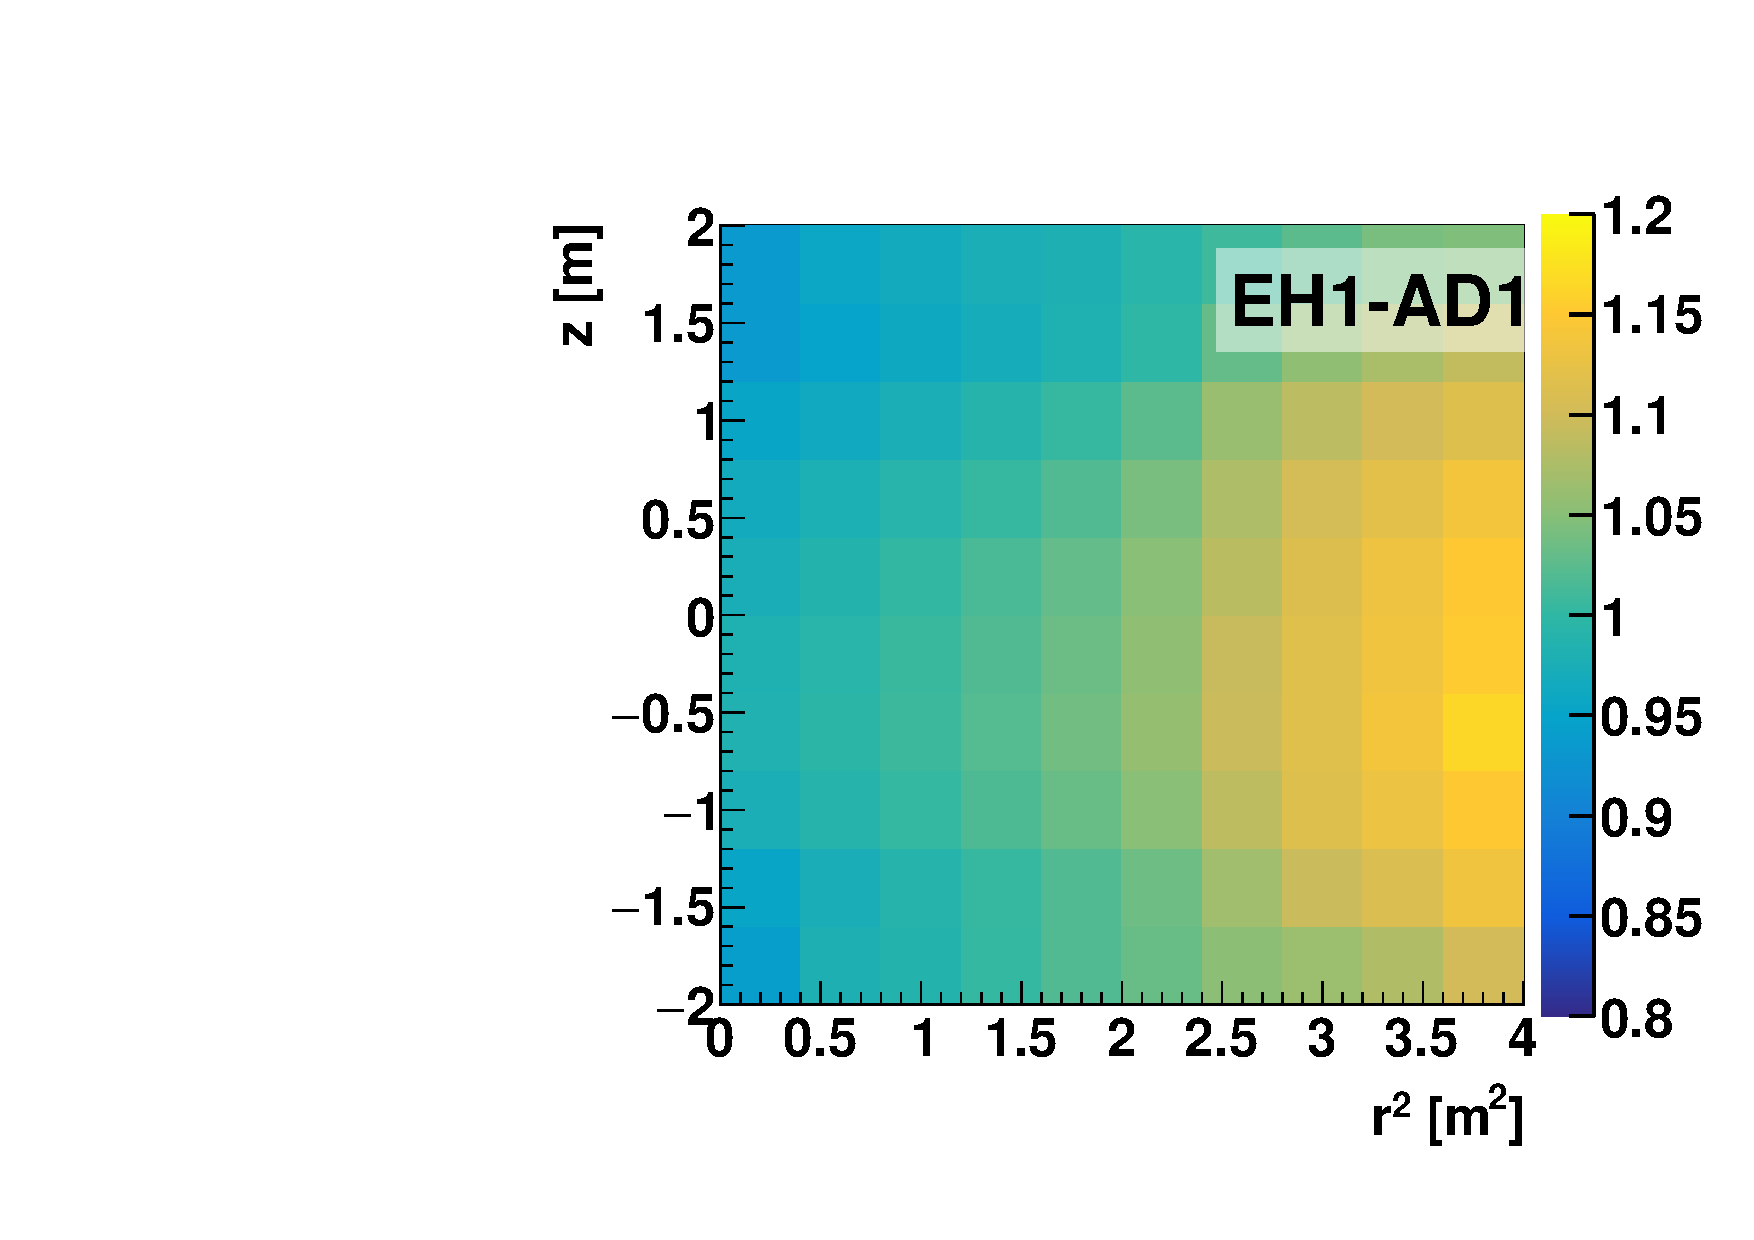
\includegraphics[width=0.4\textwidth]{ch_reconstruction/nonuniformity_map}
    \caption{
        Nonuniformity corrections based on the energy of spallation neutrons
        capturing on Gd and H.
        Plot based on data from \cite{nonuniformity2}.
    }
    \label{fig:nonuniformity_map}
\end{figure}

The Earth's magnetic field caused a nonuniformity
as a function of azimuthal angle $\phi$ of approximately \SI{1}{\percent}.
A model was constructed to account for this effect:
\begin{equation}
    f_{\text{pos}}(\phi) = 1 + \alpha\sin(\phi-\phi_0),
\end{equation}
where $\alpha$ and $\phi_0$ were determined from fitting to spallation neutron captures
in a similar fashion as with the $r$--$z$ nonuniformity.

Over time, the nonuniformity evolved in different regions of the ADs,
attributable mostly to a slight degradation in the attenuation length of the LS
and GdLS \cite{nonuniformity3}.
The evolution was quantified by examining the spallation neutron capture energy
as a function of radial position and time.
As shown in \cref{fig:time_dep_nonunif}, a clear linear change is visible
for each bin of radial position \cite{nonuniformity1}, which was parametrized as
\begin{equation}
    f_{\text{pos}}(t, r) = (\beta_0 + \beta_1r^2)t.
\end{equation}
All ADs showed a similar trend, so a combined fit was performed,
yielding values of $\beta_0 + \beta_1r^2$ between
\SIlist[retain-explicit-plus]{-0.12;+0.4}{\percent} per year.

\begin{figure}
    \centering
    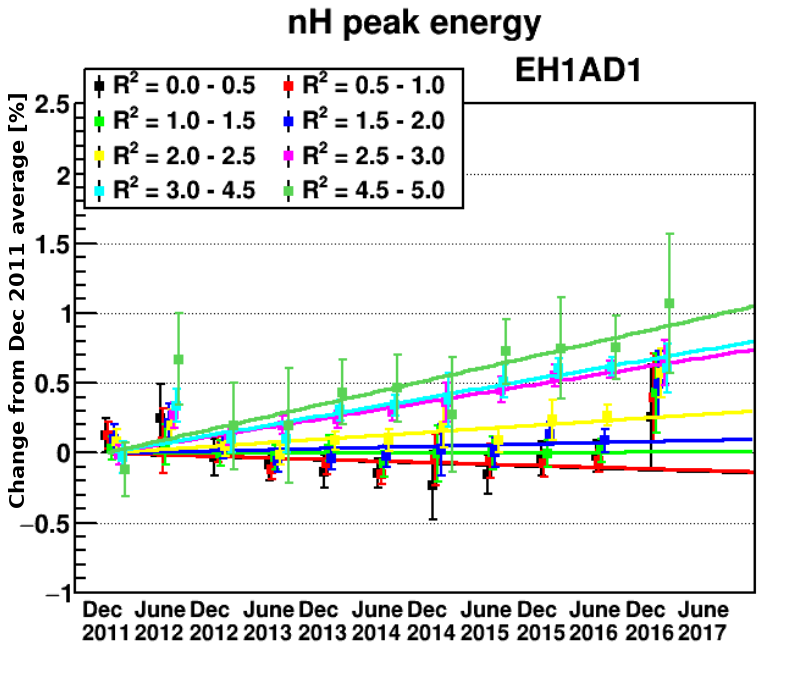
\includegraphics[width=0.4\textwidth]{ch_reconstruction/time_dep_nonunif}
    \caption{
        Relative change over time in energy for spallation neutrons capturing on H.
        Each color is a different range of event radius.
        The correction coefficients $\beta_0$ and $\beta_1$ are determined
        from a fit of the slope as a function of radius.
        Figure taken from \cite{nonuniformity4}.
    }
    \label{fig:time_dep_nonunif}
\end{figure}
